% =========================================================================== %

\begin{frame}[t,plain]
\titlepage
\end{frame}

% =========================================================================== %

\begin{frame}[fragile]{Recap}
%
\begin{itemize}
\item Datei-Management
	\begin{itemize}
	\item Zugriff über \emph{handles}:\tabto{4cm} \texttt{FILE * fp = fopen("filename", "mode");}
	\item Modi: Lesen (\texttt{r}), Schreiben (\texttt{w}), Anhängen (\texttt{a})
	\item Schreiben mit \texttt{fprintf} oder \texttt{fwrite}
	\item Lesen mit \texttt{fscanf} oder \texttt{fread}
	\item Schließen/Datei freigeben mit \texttt{fclose}
	\end{itemize}
\item Rekursion
	\begin{itemize}
	\item Funktionen, die sich selbst aufrufen
	\item Zerlegung in einfachere Unterprobleme
	\item Eigener Scope für jede Instanz
	\end{itemize}
\end{itemize}
%
\begin{center}
	\emph{Noch Fragen?}
\end{center}
%
\end{frame}

% =========================================================================== %

\begin{frame}{Script}

\begin{itemize}
\item Kapitel 17
	\begin{itemize}
	\item 17.1. Ausgangslage: Klassische Arrays
	\item 17.2. Verknüpfung mit seinen Nachbarn: Linked Lists
	\item 17.3. Aufbau einer Bibliothek zur Verwaltung von Linked Lists
	\item 17.4. Einsatzbereiche der Linked List: Vor- und Nachteile 
	\end{itemize}
\end{itemize}

\end{frame}

% =========================================================================== %

\begin{frame}[fragile]{Linked List: Ausgangsproblem}
%
\begin{columns}[T]
\column{.4\linewidth}
\vspace{-6pt}
\begin{itemize}
\item Aufgabe: Füge Element in Liste ein
\item Nötige Schritte:
	\begin{itemize}
	\item Mehr Speicherplatz allozieren
	\item Elemente \enquote{um einen Platz verschieben}
	\item Neues Element schreiben
	\end{itemize}
\item Bei häufigem Einfügen oder großen Datenmengen: Langsam
\end{itemize}
%
\column{.6\linewidth}
\vspace{-15pt}
\begin{codebox}[Beispiel: Wert Einfügen]
\begin{minted}[fontsize=\scriptsize, linenos]{c}
int * insert(int * lst, int len,
             int pos, int new)
{
   lst = realloc(lst, 
                 (len + 1) * sizeof(int));
   if (!lst) {
      printf("failure.\n"); 
      return NULL;
   }
   
   for (int i = len; i > pos; i--) {
      lst[i] = lst[i-1];
   }
   
   lst[pos] = new;
   return lst;
}
\end{minted}
\end{codebox}
\end{columns}

%
\end{frame}

% =========================================================================== %

\begin{frame}{Linked Lists: Grundidee}
%
\begin{itemize}
\item Daten nicht mehr \emph{konsekutiv} (direkt aufeinander folgend)
\item Sondern: \enquote{irgendwo} im Speicher
\item Aber: Paar aus \enquote{Nutzdaten} und \enquote{Nachfolger-Adresse}
\item[\Thus] Von einem Element aus alle seine Nachfolger auffindbar
\item[\Thus] Nicht aber die Vorgänger
\item[\Thus] Sonderrolle erstes Element
\end{itemize}
%
\end{frame}

% =========================================================================== %

\begin{frame}[fragile]
%
\begin{codebox}[Datentyp für Elemente einer Linked List]
\begin{minted}[linenos, fontsize=\scriptsize]{c}
typedef struct listElement_struct {
  int                         data;   // Nutzdaten
  struct listElement_struct * next;   // Nachfolger-Adresse
} listElement_t;
\end{minted}
\end{codebox}
%
\begin{tcolorbox}[title=Visualisierung: Verkettete Liste]
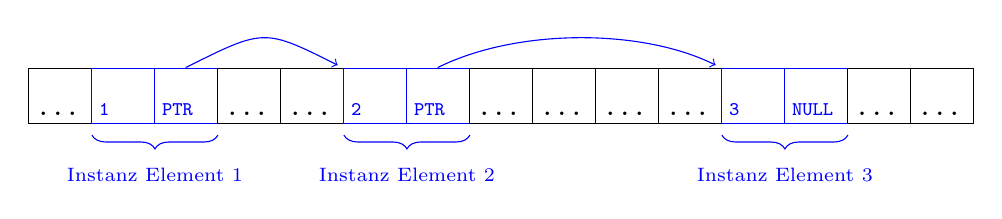
\begin{tikzpicture}
  [ 
    cell/.style={text width=6mm,
    text height=5mm, draw=black, inner sep=1mm},
    ld/.style={draw=blue,shorten >=2pt,->}
  ]
  \node (c01) at ( 0.0,0) [cell]       {\ttfamily \ldots};
  \node (c02) at ( 0.8,0) [cell, blue] {\ttfamily \scriptsize 1};
  \node (c03) at ( 1.6,0) [cell, blue] {\ttfamily \scriptsize PTR};
  \node (c04) at ( 2.4,0) [cell]       {\ttfamily \ldots};
  \node (c05) at ( 3.2,0) [cell]       {\ttfamily \ldots};
  \node (c06) at ( 4.0,0) [cell, blue] {\ttfamily \scriptsize 2};
  \node (c07) at ( 4.8,0) [cell, blue] {\ttfamily \scriptsize PTR};
  \node (c08) at ( 5.6,0) [cell]       {\ttfamily \ldots};
  \node (c09) at ( 6.4,0) [cell]       {\ttfamily \ldots};
  \node (c10) at ( 7.2,0) [cell]       {\ttfamily \ldots};
  \node (c11) at ( 8.0,0) [cell]       {\ttfamily \ldots};
  \node (c12) at ( 8.8,0) [cell, blue] {\ttfamily \scriptsize 3};
  \node (c13) at ( 9.6,0) [cell, blue] {\ttfamily \scriptsize NULL};
  \node (c14) at (10.4,0) [cell]       {\ttfamily \ldots};
  \node (c15) at (11.2,0) [cell]       {\ttfamily \ldots};
  
  \draw [ld] (c03.north) .. controls +(1.0,0.5) and +(-1.0, 0.5) .. (c06.north west);
  \draw [ld] (c07.north) .. controls +(1.0,0.5) and +(-1.0, 0.5) .. (c12.north west);
  
  \draw [decorate, decoration={brace, amplitude=5pt, mirror}, xshift=-4pt, yshift=0pt, blue]
  		(0.55, -0.5) -- (2.15, -0.5) 
  		node [midway, yshift=-0.5cm]
		(I1) {\scriptsize Instanz Element 1};
  \draw [decorate, decoration={brace, amplitude=5pt, mirror}, xshift=-4pt, yshift=0pt, blue]
  		(3.75, -0.5) -- (5.35, -0.5) 
  		node [midway, yshift=-0.5cm]
		(I2) {\scriptsize Instanz Element 2};
  \draw [decorate, decoration={brace, amplitude=5pt, mirror}, xshift=-4pt, yshift=0pt, blue]
  		(8.55, -0.5) -- (10.15, -0.5) 
  		node [midway, yshift=-0.5cm]
		(I3) {\scriptsize Instanz Element 3};
\end{tikzpicture}

\vspace{6pt}
Listenende? Lasse \texttt{next} auf ungültige Adresse zeigen: \texttt{NULL}
\end{tcolorbox}
%
\end{frame}

% =========================================================================== %

\begin{frame}[fragile]
%
\begin{tcolorbox}[title=Visualisierung: Einfügen in eine verketteten Liste]
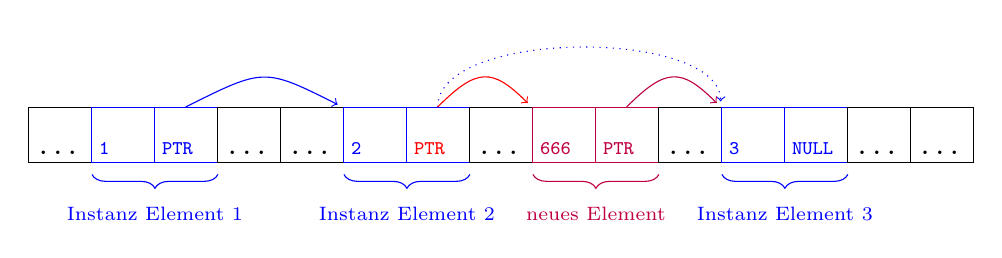
\begin{tikzpicture}
  [ 
    cell/.style={text width=6mm,
    text height=5mm, draw=black, inner sep=1mm},
    ld/.style={draw=blue,shorten >=2pt,->}
  ]
  \node (c01) at ( 0.0,0) [cell]         {\ttfamily \ldots};
  \node (c02) at ( 0.8,0) [cell, blue]   {\ttfamily \scriptsize 1};
  \node (c03) at ( 1.6,0) [cell, blue]   {\ttfamily \scriptsize PTR};
  \node (c04) at ( 2.4,0) [cell]         {\ttfamily \ldots};
  \node (c05) at ( 3.2,0) [cell]         {\ttfamily \ldots};
  \node (c06) at ( 4.0,0) [cell, blue]   {\ttfamily \scriptsize 2};
  \node (c07) at ( 4.8,0) [cell, blue]   {\ttfamily \scriptsize \textcolor{red}{PTR}};
  \node (c08) at ( 5.6,0) [cell]         {\ttfamily \ldots};
  \node (c09) at ( 6.4,0) [cell, purple] {\ttfamily \scriptsize 666};
  \node (c10) at ( 7.2,0) [cell, purple] {\ttfamily \scriptsize PTR};
  \node (c11) at ( 8.0,0) [cell]         {\ttfamily \ldots};
  \node (c12) at ( 8.8,0) [cell, blue]   {\ttfamily \scriptsize 3};
  \node (c13) at ( 9.6,0) [cell, blue]   {\ttfamily \scriptsize NULL};
  \node (c14) at (10.4,0) [cell]         {\ttfamily \ldots};
  \node (c15) at (11.2,0) [cell]         {\ttfamily \ldots};
  
  \draw [ld]         (c03.north) .. controls +(1.0,0.5) and +(-1.0, 0.5) .. (c06.north west);
  \draw [ld, dotted] (c07.north) .. controls +(0.0,1.0) and +(-0.0, 1.0) .. (c12.north west);
  \draw [ld, red]    (c07.north) .. controls +(0.5,0.5) and +(-0.5, 0.5) .. (c09.north west);
  \draw [ld, purple] (c10.north) .. controls +(0.5,0.5) and +(-0.5, 0.5) .. (c12.north west);

  \draw [decorate, decoration={brace, amplitude=5pt, mirror}, xshift=-4pt, yshift=0pt, blue]
  		(0.55, -0.5) -- (2.15, -0.5) 
  		node [midway, yshift=-0.5cm]
		(I1) {\scriptsize Instanz Element 1};
  \draw [decorate, decoration={brace, amplitude=5pt, mirror}, xshift=-4pt, yshift=0pt, blue]
  		(3.75, -0.5) -- (5.35, -0.5) 
  		node [midway, yshift=-0.5cm]
		(I2) {\scriptsize Instanz Element 2};
  \draw [decorate, decoration={brace, amplitude=5pt, mirror}, xshift=-4pt, yshift=0pt, blue]
  		(8.55, -0.5) -- (10.15, -0.5) 
  		node [midway, yshift=-0.5cm]
		(I3) {\scriptsize Instanz Element 3};
  \draw [decorate, decoration={brace, amplitude=5pt, mirror}, xshift=-4pt, yshift=0pt, purple]
  		(6.15, -0.5) -- (7.75, -0.5) 
  		node [midway, yshift=-0.5cm]
		(I4) {\scriptsize neues Element};
\end{tikzpicture}
%
\begin{itemize}
\item Neues Element vorbereiten
\item Zeigt auf Nachfolger
\item Pointer des Vorgängers updaten
\item[\Thus] Kein Kopieren/Verschieben nötig!
\end{itemize}
\end{tcolorbox}
%
\end{frame}

% =========================================================================== %

\begin{frame}[fragile]
%
\begin{tcolorbox}[title=Visualisierung: Einfügen an das Ende einer verketteten Liste]
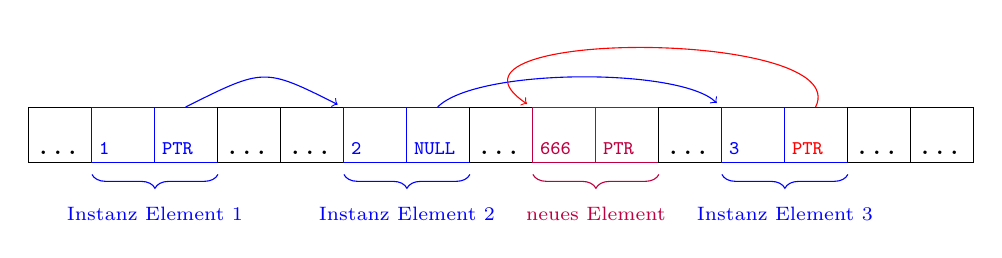
\begin{tikzpicture}
  [ 
    cell/.style={text width=6mm,
    text height=5mm, draw=black, inner sep=1mm},
    ld/.style={draw=blue,shorten >=2pt,->}
  ]
  \node (c01) at ( 0.0,0) [cell]         {\ttfamily \ldots};
  \node (c02) at ( 0.8,0) [cell, blue]   {\ttfamily \scriptsize 1};
  \node (c03) at ( 1.6,0) [cell, blue]   {\ttfamily \scriptsize PTR};
  \node (c04) at ( 2.4,0) [cell]         {\ttfamily \ldots};
  \node (c05) at ( 3.2,0) [cell]         {\ttfamily \ldots};
  \node (c06) at ( 4.0,0) [cell, blue]   {\ttfamily \scriptsize 2};
  \node (c07) at ( 4.8,0) [cell, blue]   {\ttfamily \scriptsize NULL};
  \node (c08) at ( 5.6,0) [cell]         {\ttfamily \ldots};
  \node (c09) at ( 6.4,0) [cell, purple] {\ttfamily \scriptsize 666};
  \node (c10) at ( 7.2,0) [cell, purple] {\ttfamily \scriptsize PTR};
  \node (c11) at ( 8.0,0) [cell]         {\ttfamily \ldots};
  \node (c12) at ( 8.8,0) [cell, blue]   {\ttfamily \scriptsize 3};
  \node (c13) at ( 9.6,0) [cell, blue]   {\ttfamily \scriptsize \textcolor{red}{PTR}};
  \node (c14) at (10.4,0) [cell]         {\ttfamily \ldots};
  \node (c15) at (11.2,0) [cell]         {\ttfamily \ldots};
  
  \draw [ld]         (c03.north) .. controls +(1.0,0.5) and +(-1.0, 0.5) .. (c06.north west);
  \draw [ld]         (c07.north) .. controls +(0.5,0.5) and +(-0.5, 0.5) .. (c12.north west);
  \draw [ld, red]    (c13.north) .. controls +(0.5,1.0) and +(-1.5, 1.0) .. (c09.north west);

  \draw [decorate, decoration={brace, amplitude=5pt, mirror}, xshift=-4pt, yshift=0pt, blue]
  		(0.55, -0.5) -- (2.15, -0.5) 
  		node [midway, yshift=-0.5cm]
		(I1) {\scriptsize Instanz Element 1};
  \draw [decorate, decoration={brace, amplitude=5pt, mirror}, xshift=-4pt, yshift=0pt, blue]
  		(3.75, -0.5) -- (5.35, -0.5) 
  		node [midway, yshift=-0.5cm]
		(I2) {\scriptsize Instanz Element 2};
  \draw [decorate, decoration={brace, amplitude=5pt, mirror}, xshift=-4pt, yshift=0pt, blue]
  		(8.55, -0.5) -- (10.15, -0.5) 
  		node [midway, yshift=-0.5cm]
		(I3) {\scriptsize Instanz Element 3};
  \draw [decorate, decoration={brace, amplitude=5pt, mirror}, xshift=-4pt, yshift=0pt, purple]
  		(6.15, -0.5) -- (7.75, -0.5) 
  		node [midway, yshift=-0.5cm]
		(I4) {\scriptsize neues Element};
\end{tikzpicture}
%
\begin{itemize}
\item Neues Element vorbereiten
\item Zeigt auf \texttt{NULL}
\item Pointer des vormals letzten Elements updaten
\end{itemize}
\end{tcolorbox}
%
\end{frame}

% =========================================================================== %

\begin{frame}
%
\begin{tcolorbox}[title=Visualisierung: Einfügen an den Anfang einer verketteten Liste]
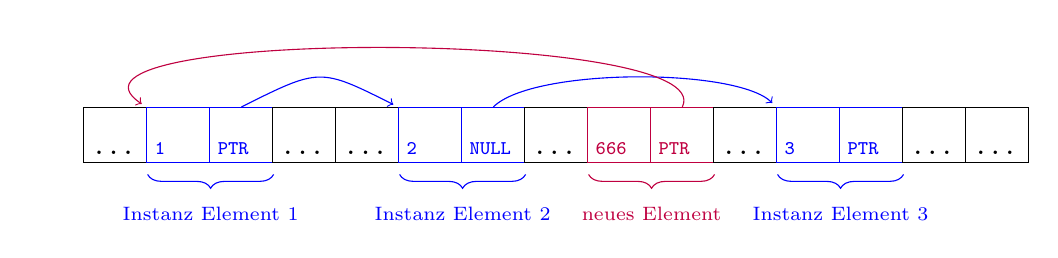
\begin{tikzpicture}
  [ 
    cell/.style={text width=6mm,
    text height=5mm, draw=black, inner sep=1mm},
    ld/.style={draw=blue,shorten >=2pt,->}
  ]
  \node (c01) at ( 0.0,0) [cell]         {\ttfamily \ldots};
  \node (c02) at ( 0.8,0) [cell, blue]   {\ttfamily \scriptsize 1};
  \node (c03) at ( 1.6,0) [cell, blue]   {\ttfamily \scriptsize PTR};
  \node (c04) at ( 2.4,0) [cell]         {\ttfamily \ldots};
  \node (c05) at ( 3.2,0) [cell]         {\ttfamily \ldots};
  \node (c06) at ( 4.0,0) [cell, blue]   {\ttfamily \scriptsize 2};
  \node (c07) at ( 4.8,0) [cell, blue]   {\ttfamily \scriptsize NULL};
  \node (c08) at ( 5.6,0) [cell]         {\ttfamily \ldots};
  \node (c09) at ( 6.4,0) [cell, purple] {\ttfamily \scriptsize 666};
  \node (c10) at ( 7.2,0) [cell, purple] {\ttfamily \scriptsize PTR};
  \node (c11) at ( 8.0,0) [cell]         {\ttfamily \ldots};
  \node (c12) at ( 8.8,0) [cell, blue]   {\ttfamily \scriptsize 3};
  \node (c13) at ( 9.6,0) [cell, blue]   {\ttfamily \scriptsize PTR};
  \node (c14) at (10.4,0) [cell]         {\ttfamily \ldots};
  \node (c15) at (11.2,0) [cell]         {\ttfamily \ldots};
  
  \draw [ld]         (c03.north) .. controls +(1.0,0.5) and +(-1.0, 0.5) .. (c06.north west);
  \draw [ld]         (c07.north) .. controls +(0.5,0.5) and +(-0.5, 0.5) .. (c12.north west);
  \draw [ld, purple] (c10.north) .. controls +(0.5,1.0) and +(-1.5, 1.0) .. (c02.north west);

  \draw [decorate, decoration={brace, amplitude=5pt, mirror}, xshift=-4pt, yshift=0pt, blue]
  		(0.55, -0.5) -- (2.15, -0.5) 
  		node [midway, yshift=-0.5cm]
		(I1) {\scriptsize Instanz Element 1};
  \draw [decorate, decoration={brace, amplitude=5pt, mirror}, xshift=-4pt, yshift=0pt, blue]
  		(3.75, -0.5) -- (5.35, -0.5) 
  		node [midway, yshift=-0.5cm]
		(I2) {\scriptsize Instanz Element 2};
  \draw [decorate, decoration={brace, amplitude=5pt, mirror}, xshift=-4pt, yshift=0pt, blue]
  		(8.55, -0.5) -- (10.15, -0.5) 
  		node [midway, yshift=-0.5cm]
		(I3) {\scriptsize Instanz Element 3};
  \draw [decorate, decoration={brace, amplitude=5pt, mirror}, xshift=-4pt, yshift=0pt, purple]
  		(6.15, -0.5) -- (7.75, -0.5) 
  		node [midway, yshift=-0.5cm]
		(I4) {\scriptsize neues Element};
\end{tikzpicture}
%
\begin{itemize}
\item Neues Element mit korrektem Pointer vorbereiten
\item Einstiegspunkt ändert sich!
\end{itemize}
\end{tcolorbox}
%
\end{frame}

% =========================================================================== %

\begin{frame}
%
\begin{tcolorbox}[title=Visualisierung: Löschen aus einer verketteten Liste]
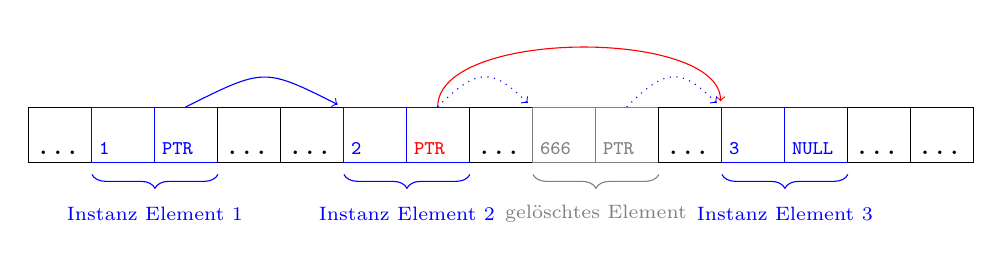
\begin{tikzpicture}
  [ 
    cell/.style={text width=6mm,
    text height=5mm, draw=black, inner sep=1mm},
    ld/.style={draw=blue,shorten >=2pt,->}
  ]

  \node (c01) at ( 0.0,0) [cell]         {\ttfamily \ldots};
  \node (c02) at ( 0.8,0) [cell, blue]   {\ttfamily \scriptsize 1};
  \node (c03) at ( 1.6,0) [cell, blue]   {\ttfamily \scriptsize PTR};
  \node (c04) at ( 2.4,0) [cell]         {\ttfamily \ldots};
  \node (c05) at ( 3.2,0) [cell]         {\ttfamily \ldots};
  \node (c06) at ( 4.0,0) [cell, blue]   {\ttfamily \scriptsize 2};
  \node (c07) at ( 4.8,0) [cell, blue]   {\ttfamily \scriptsize \textcolor{red}{PTR}};
  \node (c08) at ( 5.6,0) [cell]         {\ttfamily \ldots};
  \node (c09) at ( 6.4,0) [cell, gray]   {\ttfamily \scriptsize 666};
  \node (c10) at ( 7.2,0) [cell, gray]   {\ttfamily \scriptsize PTR};
  \node (c11) at ( 8.0,0) [cell]         {\ttfamily \ldots};
  \node (c12) at ( 8.8,0) [cell, blue]   {\ttfamily \scriptsize 3};
  \node (c13) at ( 9.6,0) [cell, blue]   {\ttfamily \scriptsize NULL};
  \node (c14) at (10.4,0) [cell]         {\ttfamily \ldots};
  \node (c15) at (11.2,0) [cell]         {\ttfamily \ldots};
  
  \draw [ld]         (c03.north) .. controls +(1.0,0.5) and +(-1.0, 0.5) .. (c06.north west);
  \draw [ld, red]    (c07.north) .. controls +(0.0,1.0) and +(-0.0, 1.0) .. (c12.north west);
  \draw [ld, dotted] (c07.north) .. controls +(0.5,0.5) and +(-0.5, 0.5) .. (c09.north west);
  \draw [ld, dotted] (c10.north) .. controls +(0.5,0.5) and +(-0.5, 0.5) .. (c12.north west);

  \draw [decorate, decoration={brace, amplitude=5pt, mirror}, xshift=-4pt, yshift=0pt, blue]
  		(0.55, -0.5) -- (2.15, -0.5) 
  		node [midway, yshift=-0.5cm]
		(I1) {\scriptsize Instanz Element 1};
  \draw [decorate, decoration={brace, amplitude=5pt, mirror}, xshift=-4pt, yshift=0pt, blue]
  		(3.75, -0.5) -- (5.35, -0.5) 
  		node [midway, yshift=-0.5cm]
		(I2) {\scriptsize Instanz Element 2};
  \draw [decorate, decoration={brace, amplitude=5pt, mirror}, xshift=-4pt, yshift=0pt, blue]
  		(8.55, -0.5) -- (10.15, -0.5) 
  		node [midway, yshift=-0.5cm]
		(I3) {\scriptsize Instanz Element 3};
  \draw [decorate, decoration={brace, amplitude=5pt, mirror}, xshift=-4pt, yshift=0pt, gray]
  		(6.15, -0.5) -- (7.75, -0.5) 
  		node [midway, yshift=-0.5cm]
		(I4) {\scriptsize gelöschtes Element};
\end{tikzpicture}
%
\begin{itemize}
\item Pointer des Vorgängers updaten
\item Speicher freigeben
\item Ähnliche Sonderfälle für Listenanfang und Listenende
\item[\Thus] Wieder: Kein Kopieren/Verschieben!
\end{itemize}
\end{tcolorbox}
%
\end{frame}

% =========================================================================== %

\begin{frame}[fragile]{Problem Einstiegspunkt}
%
\begin{columns}[T]
\column{.5\linewidth}
\begin{itemize}
\item Einfügen und Löschen kann Einstiegspunkt verändern
\item Funktionen, die diese Aufgaben übernehmen müssen diese Information weiterleiten
\item Verwaltungsvariable muss sich ändern
\item Lösung: \emph{Zwei} Datentypen
	\begin{itemize}
	\item Listenelemente
	\item Verwaltungs-Variable
	\end{itemize}
\item Vorteil: Adresse von Verwaltungsvariable ändert sich nie!
\end{itemize}
%
\column{.5\linewidth}
\vspace{-5pt}
\begin{codebox}[Datentypen für Listenelemente und Verwaltungsvariable einer Linked List]
\begin{minted}[linenos, fontsize=\scriptsize]{c}
typedef struct listElement_struct {
  void *                      data;
  struct listElement_struct * next;
} listElement_t;

typedef struct {
  listElement_t * first;
  int             size;
  
  int             memoryAutoManaged;
  void (*printElement)(void *);
} linkedList_t;
\end{minted}
\end{codebox}
\end{columns}
%
\end{frame}

% =========================================================================== %

\begin{frame}[fragile]{Problem Generalisierung}
%
\begin{columns}[T]
\column{.5\linewidth}
\begin{itemize}
\item Bisher: Nur Listen von \inC{int}s
\item Viel Aufwand; wir wollen nicht für jeden Datentyp neue LinkedLists schreiben!
\item[\Thus] Nutzdaten sind \emph{Pointer auf \inC{void}}
\end{itemize}

\vspace{3pt}
\begin{itemize}
\item Benutzerdefinierte Interpretation des Speicherbereichs am Zielort
\item[\Thus] \texttt{print}-Methode
\end{itemize}

\vspace{3pt}
\begin{itemize}
\item Wir als Programmierer*innen sind für die Speicherverwaltung zuständig
\item[\Thus] Automatisierung an/abschalten
\end{itemize}

\column{.5\linewidth}
\vspace{-5pt}
\begin{codebox}[Datentypen für Listenelemente und Verwaltungsvariable einer Linked List]
\begin{minted}[linenos, fontsize=\scriptsize]{c}
typedef struct listElement_struct {
  void *                      data;
  struct listElement_struct * next;
} listElement_t;

typedef struct {
  listElement_t * first;
  int             size;
  
  int             memoryAutoManaged;
  void (*printElement)(void *);
} linkedList_t;
\end{minted}
\end{codebox}
\end{columns}
%
\end{frame}

% =========================================================================== %

\begin{frame}
%
\begin{tcolorbox}[title=Visualisierung: Struktur mit Verwaltungsvariable]
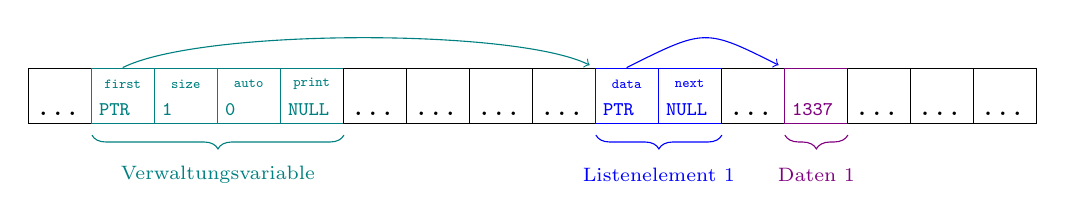
\begin{tikzpicture}
  [ 
    cell/.style={text width=6mm,
    text height=5mm, draw=black, inner sep=1mm},
    ld/.style={draw=blue,shorten >=2pt,->}
  ]

  \node (c00) at ( 0.0,0) [cell]         {\ttfamily \ldots};
  \node (c01) at ( 0.8,0) [cell, teal]   {\ttfamily \scriptsize PTR};
  \node (c02) at ( 1.6,0) [cell, teal]   {\ttfamily \scriptsize 1};
  \node (c03) at ( 2.4,0) [cell, teal]   {\ttfamily \scriptsize 0};
  \node (c04) at ( 3.2,0) [cell, teal]   {\ttfamily \scriptsize NULL};
  \node (c05) at ( 4.0,0) [cell]         {\ttfamily \ldots};
  \node (c06) at ( 4.8,0) [cell]         {\ttfamily \ldots};
  \node (c07) at ( 5.6,0) [cell]         {\ttfamily \ldots};
  \node (c08) at ( 6.4,0) [cell]         {\ttfamily \ldots};
  \node (c09) at ( 7.2,0) [cell, blue]   {\ttfamily \scriptsize PTR};
  \node (c10) at ( 8.0,0) [cell, blue]   {\ttfamily \scriptsize NULL};
  \node (c11) at ( 8.8,0) [cell]         {\ttfamily \ldots};
  \node (c12) at ( 9.6,0) [cell, violet] {\ttfamily \scriptsize 1337};
  \node (c13) at (10.4,0) [cell]         {\ttfamily \ldots};
  \node (c14) at (11.2,0) [cell]         {\ttfamily \ldots};
  \node (c15) at (12.0,0) [cell]         {\ttfamily \ldots};

  \node (l01) at ( 0.8,.15) [teal] {\ttfamily \tiny first};
  \node (l02) at ( 1.6,.15) [teal] {\ttfamily \tiny size};
  \node (l03) at ( 2.4,.15) [teal] {\ttfamily \tiny auto};
  \node (l04) at ( 3.2,.15) [teal] {\ttfamily \tiny print};
  
  \node (l09) at ( 7.2,.15) [blue] {\ttfamily \tiny data};
  \node (l10) at ( 8.0,.15) [blue] {\ttfamily \tiny next};
  
  \draw [ld, teal]   (c01.north) .. controls +(1.0,0.5) and +(-1.0, 0.5) .. (c09.north west);
  \draw [ld, blue]   (c09.north) .. controls +(1.0,0.5) and +(-1.0, 0.5) .. (c12.north west);

  \draw [decorate, decoration={brace, amplitude=5pt, mirror}, xshift=-4pt, yshift=0pt, teal]
  		(0.55, -0.5) -- (3.75, -0.5) 
  		node [midway, yshift=-0.5cm]
		(I0) {\scriptsize Verwaltungsvariable};
  \draw [decorate, decoration={brace, amplitude=5pt, mirror}, xshift=-4pt, yshift=0pt, blue]
  		(6.95, -0.5) -- (8.55, -0.5) 
  		node [midway, yshift=-0.5cm]
		(I1) {\scriptsize Listenelement 1};
  \draw [decorate, decoration={brace, amplitude=5pt, mirror}, xshift=-4pt, yshift=0pt, violet]
  		(9.35, -0.5) -- (10.15, -0.5) 
  		node [midway, yshift=-0.5cm]
		(N1) {\scriptsize Daten 1};
\end{tikzpicture}
\end{tcolorbox}
%
\begin{tcolorbox}[title=Visualisierung: Einfügen mit Verwaltungsvariable]
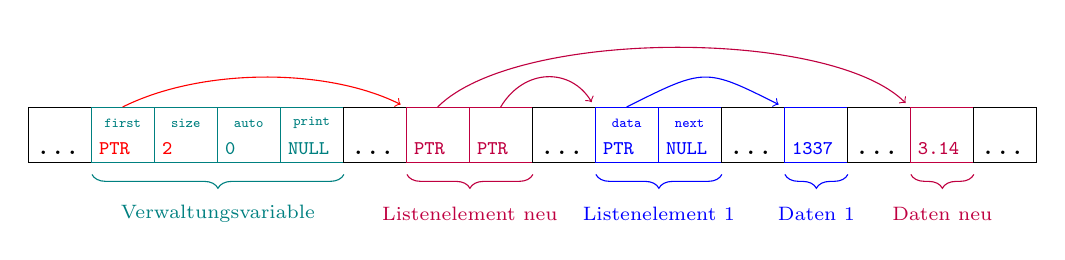
\begin{tikzpicture}
  [ 
    cell/.style={text width=6mm,
    text height=5mm, draw=black, inner sep=1mm},
    ld/.style={draw=blue,shorten >=2pt,->}
  ]

  \node (c00) at ( 0.0,0) [cell]         {\ttfamily \ldots};
  \node (c01) at ( 0.8,0) [cell, teal]   {\ttfamily \scriptsize \color{red} PTR};
  \node (c02) at ( 1.6,0) [cell, teal]   {\ttfamily \scriptsize \color{red} 2};
  \node (c03) at ( 2.4,0) [cell, teal]   {\ttfamily \scriptsize 0};
  \node (c04) at ( 3.2,0) [cell, teal]   {\ttfamily \scriptsize NULL};
  \node (c05) at ( 4.0,0) [cell]         {\ttfamily \ldots};
  \node (c06) at ( 4.8,0) [cell, purple] {\ttfamily \scriptsize PTR};
  \node (c07) at ( 5.6,0) [cell, purple] {\ttfamily \scriptsize PTR};
  \node (c08) at ( 6.4,0) [cell]         {\ttfamily \ldots};
  \node (c09) at ( 7.2,0) [cell, blue]   {\ttfamily \scriptsize PTR};
  \node (c10) at ( 8.0,0) [cell, blue]   {\ttfamily \scriptsize NULL};
  \node (c11) at ( 8.8,0) [cell]         {\ttfamily \ldots};
  \node (c12) at ( 9.6,0) [cell, blue]   {\ttfamily \scriptsize 1337};
  \node (c13) at (10.4,0) [cell]         {\ttfamily \ldots};
  \node (c14) at (11.2,0) [cell, purple] {\ttfamily \scriptsize 3.14};
  \node (c15) at (12.0,0) [cell]         {\ttfamily \ldots};

  \node (l01) at ( 0.8,.15) [teal] {\ttfamily \tiny first};
  \node (l02) at ( 1.6,.15) [teal] {\ttfamily \tiny size};
  \node (l03) at ( 2.4,.15) [teal] {\ttfamily \tiny auto};
  \node (l04) at ( 3.2,.15) [teal] {\ttfamily \tiny print};
  
  \node (l09) at ( 7.2,.15) [blue] {\ttfamily \tiny data};
  \node (l10) at ( 8.0,.15) [blue] {\ttfamily \tiny next};
  
  \draw [ld, red]    (c01.north) .. controls +(1.0,0.5) and +(-1.0, 0.5) .. (c06.north west);
  \draw [ld, blue]   (c09.north) .. controls +(1.0,0.5) and +(-1.0, 0.5) .. (c12.north west);
  \draw [ld, purple] (c07.north) .. controls +(0.3,0.5) and +(-0.3, 0.5) .. (c09.north west);
  \draw [ld, purple] (c06.north) .. controls +(1.0,1.0) and +(-1.0, 1.0) .. (c14.north west);

  \draw [decorate, decoration={brace, amplitude=5pt, mirror}, xshift=-4pt, yshift=0pt, teal]
  		(0.55, -0.5) -- (3.75, -0.5) 
  		node [midway, yshift=-0.5cm]
		(I0) {\scriptsize Verwaltungsvariable};
  \draw [decorate, decoration={brace, amplitude=5pt, mirror}, xshift=-4pt, yshift=0pt, purple]
  		(4.55, -0.5) -- (6.15, -0.5) 
  		node [midway, yshift=-0.5cm]
		(I1) {\scriptsize Listenelement neu};
  \draw [decorate, decoration={brace, amplitude=5pt, mirror}, xshift=-4pt, yshift=0pt, blue]
  		(6.95, -0.5) -- (8.55, -0.5) 
  		node [midway, yshift=-0.5cm]
		(I1) {\scriptsize Listenelement 1};
  \draw [decorate, decoration={brace, amplitude=5pt, mirror}, xshift=-4pt, yshift=0pt, blue]
  		(9.35, -0.5) -- (10.15, -0.5) 
  		node [midway, yshift=-0.5cm]
		(N1) {\scriptsize Daten 1};
  \draw [decorate, decoration={brace, amplitude=5pt, mirror}, xshift=-4pt, yshift=0pt, purple]
  		(10.95, -0.5) -- (11.75, -0.5) 
  		node [midway, yshift=-0.5cm]
		(N1) {\scriptsize Daten neu};
\end{tikzpicture}
\end{tcolorbox}
%
\end{frame}

% =========================================================================== %

\begin{frame}[fragile]{Warum \texttt{memoryAutoManaged}?}
%
\begin{itemize}
\item Beispiel: Liste von Strings
\item Erinnerung: \texttt{String} \thus Array von \inC{char}s
\item Können als \emph{literal strings} oder in automatischen Arrays vorliegen 
	\begin{itemize}
	\item \inC{"literal string"}
	\item \inC{char string[100];}
	\item[\Thus] kein \texttt{free} erlaubt!
	\end{itemize}
\item Oder als \emph{dynamische Arrays}
	\begin{itemize}
	\item \inC{char string = malloc(100);}
	\item[\Thus] Braucht zwingend \texttt{free}!
	\end{itemize}
\item Wir \texttt{free\_linkedList(list);}
\item[\Thus] soll \texttt{free\_linkedList} \texttt{free} aufrufen?
\end{itemize}
%
\end{frame}

% =========================================================================== %

\begin{frame}
%
\begin{center}
(Codebeispiel: Linked List)
\end{center}
%
\end{frame}

% =========================================================================== %

\begin{frame}{Anmerkungen zur Anwendung von Linked Lists}
%
\begin{itemize}
\item \emph{FIFO}: First in First Out
	\begin{itemize}
	\item Schnelles Einfügen/Löschen vom Anfang der Liste
	\item Mitte der Liste: \enquote{Durchhangeln} nötig
	\end{itemize}
\item Iteration über \emph{alle} Listenelemente: Leicht umsetzbar
\item Sortieren: Schwierig
\item[$\Rightarrow$] Auf spezielle Anwendungsfälle zugeschnitten
\item Andere Speicherstrukturen für andere Fälle
	\begin{itemize}
	\item Doubly Linked Lists (\enquote{LIFO}: Last In First Out)
	\item Binary Search Trees
	\item Red/Black-Trees
	\item \ldots
	\end{itemize}
\item Vorlesung \emph{Algorithmen und Datenstrukturen}
\end{itemize}
%
\end{frame}